\documentclass[a4paper,12pt]{article}
\usepackage[top = 2.5cm, bottom = 2.5cm, left = 2.5cm, right = 2.5cm]{geometry}
% Unfortunately, LaTeX has a hard time interpreting German Umlaute. The following two lines and packages should help. If it doesn't work for you please let me know.
\usepackage[T1]{fontenc}
\usepackage[utf8]{inputenc}
\usepackage{tikz}
\usepackage[outercaption]{sidecap}  
% The following two packages - multirow and booktabs - are needed to create nice looking tables.
\usepackage{multirow} % Multirow is for tables with multiple rows within one cell.
\usepackage{booktabs} % For even nicer tables.
% As we usually want to include some plots (.pdf files) we need a package for that.
\usepackage{graphicx}
% The default setting of LaTeX is to indent new paragraphs. This is useful for articles. But not really nice for homework problem sets. The following command sets the indent to 0.
\usepackage[spanish]{babel}
\usepackage{setspace}
\setlength{\parindent}{0in}
% Package to place figures where you want them.
\usepackage{float}
% The fancyhdr package let's us create nice headers.
\usepackage{fancyhdr}
\usepackage{amsmath}
\usepackage{amssymb}
\usepackage{natbib}
\usepackage{graphicx}
\usepackage{subcaption}
%propios---
\usepackage{etoolbox}
\AtBeginEnvironment{align}{\setcounter{equation}{0}}

\newcommand{\al}{\alpha}
\newcommand{\be}{\beta}
\newcommand{\g}{\gamma}
\newcommand{\p}{\phi}
\newcommand{\up}{\upsilon}
\newcommand{\s}[1]{\{#1\}}
\newcommand{\ie}[4]{\int_{#1}^{#2} #3 \, d{#4}}
\newcommand{\la}[1]{\mathcal{L}[#1]}
\newcommand{\lai}[1]{\mathcal{L}^{-1}[#1]}
\newcommand{\suma}[3]{\sum_{#1}^{#2}{#3}}
\newcommand{\mi}[1]{&& #1 &&}
\newcommand{\bv}[1]{\langle #1 \rangle}
\newcommand{\uvec}[1]{\boldsymbol{\hat{\textbf{#1}}}}
\newcommand{\vf}[3]{#1\uvec{i}#2\uvec{j}#3\uvec{k}}
\newcommand{\vfd}[2]{#1\uvec{i}#2\uvec{j}}
\newcommand{\ej}[1]{\begin{exercise}
\begin{align}
    #1
\end{align}
\end{exercise}
}
\newcommand{\dn}[1]{\begin{definition}
\begin{align}
    #1
\end{align}
\end{definition}
}
\newcommand{\ta}[1]{\begin{theorem}
\begin{align}
    #1
\end{align}
\end{theorem}
}
\newcommand{\derivada}[2]{\frac{d#1}{d#2}}

\newcommand{\ieo}[4]{\oint_{#1}^{#2} #3 \, d{#4}}
\newcommand{\ied}[4]{\int_{#1}^{#2}\int_{#3}^{#4}}

\pagestyle{fancy}

\fancyhf{}

\lhead{\footnotesize Física 3: HT 4}
\rhead{\footnotesize Rompich}
\cfoot{\footnotesize \thepage}

\begin{document}
    \thispagestyle{empty} % This command disables the header on the first page.

    \begin{tabular}{p{15.5cm}} % This is a simple tabular environment to align your text nicely
    \begin{tabbing}
    Universidad del Valle de Guatemala \\ Facultad de Ciencias y Humanidades\\Departamento de Física \\7 de noviembre de 2020  \\
    Rudik R. Rompich\   - Carné: 19857\\
    \end{tabbing}
    Física 3 - Ing. Luis Mijangos \\
    \hline % \hline produces horizontal lines.
    \\
    \end{tabular} % Our tabular environment ends here.
    \vspace*{0.3cm} % Now we want to add some vertical space in between the line and our title.
    \begin{center} % Everything within the center environment is centered.
    {\Large \bf HT 3: FUERZA Y TORQUE MAGNÉTICO} % <---- Don't forget to put in the right number
        \vspace{2mm}
    \end{center}
    \vspace{0.4cm}
    

    
    
\textbf{Problema 1}

La Tierra es bombardeada por partículas provenientes del espacio exterior denominadas muones, cuya carga es idéntica a la de un electrón, pero son mucho más pesadas que éste $\left(m=1.88 \times 10^{-28} \mathrm{kg}\right)$. Suponga que en un laboratorio se establece un intenso campo magnético $(B=0.50 \mathrm{T}) \mathrm{y}$ que muones entran en este campo con una velocidad de $3.0 \times 10^{6} \mathrm{m} / \mathrm{s}$ formando un ángulo recto con el campo. ¿Cuál es el radio de la órbita resultante del muón?\\\\
\textit{Solución}
\begin{center}


\tikzset{every picture/.style={line width=0.75pt}} %set default line width to 0.75pt        

\begin{tikzpicture}[x=0.75pt,y=0.75pt,yscale=-1,xscale=1]
%uncomment if require: \path (0,350); %set diagram left start at 0, and has height of 350

%Shape: Circle [id:dp2519545521982379] 
\draw  [dash pattern={on 6.75pt off 4.5pt}][line width=2.25]  (224,165.75) .. controls (224,111.76) and (267.76,68) .. (321.75,68) .. controls (375.74,68) and (419.5,111.76) .. (419.5,165.75) .. controls (419.5,219.74) and (375.74,263.5) .. (321.75,263.5) .. controls (267.76,263.5) and (224,219.74) .. (224,165.75) -- cycle ;
%Straight Lines [id:da41741408800252666] 
\draw [line width=1.5]    (321.75,68) -- (424.5,70.91) ;
\draw [shift={(427.5,71)}, rotate = 181.62] [color={rgb, 255:red, 0; green, 0; blue, 0 }  ][line width=1.5]    (14.21,-4.28) .. controls (9.04,-1.82) and (4.3,-0.39) .. (0,0) .. controls (4.3,0.39) and (9.04,1.82) .. (14.21,4.28)   ;
%Straight Lines [id:da21207654727547398] 
\draw [line width=1.5]    (321.75,68) -- (322.47,144) ;
\draw [shift={(322.5,147)}, rotate = 269.46] [color={rgb, 255:red, 0; green, 0; blue, 0 }  ][line width=1.5]    (14.21,-4.28) .. controls (9.04,-1.82) and (4.3,-0.39) .. (0,0) .. controls (4.3,0.39) and (9.04,1.82) .. (14.21,4.28)   ;
%Straight Lines [id:da2524227401072936] 
\draw  [dash pattern={on 4.5pt off 4.5pt}]  (321.75,165.75) -- (386.5,235) ;
%Shape: Circle [id:dp05467992503115027] 
\draw  [fill={rgb, 255:red, 255; green, 0; blue, 0 }  ,fill opacity=1 ] (313.5,68) .. controls (313.5,63.44) and (317.19,59.75) .. (321.75,59.75) .. controls (326.31,59.75) and (330,63.44) .. (330,68) .. controls (330,72.56) and (326.31,76.25) .. (321.75,76.25) .. controls (317.19,76.25) and (313.5,72.56) .. (313.5,68) -- cycle ;
%Straight Lines [id:da456890387380657] 
\draw    (292.5,29) -- (314.71,55.47) ;
\draw [shift={(316,57)}, rotate = 229.99] [color={rgb, 255:red, 0; green, 0; blue, 0 }  ][line width=0.75]    (10.93,-3.29) .. controls (6.95,-1.4) and (3.31,-0.3) .. (0,0) .. controls (3.31,0.3) and (6.95,1.4) .. (10.93,3.29)   ;
%Straight Lines [id:da8857612554846259] 
\draw [color={rgb, 255:red, 208; green, 2; blue, 27 }  ,draw opacity=1 ]   (204.6,232.8) -- (225.6,253.8) ;
%Straight Lines [id:da4004393305000622] 
\draw [color={rgb, 255:red, 208; green, 2; blue, 27 }  ,draw opacity=1 ]   (205.1,253.8) -- (225.1,232.8) ;
%Straight Lines [id:da21448685599257167] 
\draw [color={rgb, 255:red, 208; green, 2; blue, 27 }  ,draw opacity=1 ]   (252.6,232.8) -- (272.6,253.8) ;
%Straight Lines [id:da19833635685402284] 
\draw [color={rgb, 255:red, 208; green, 2; blue, 27 }  ,draw opacity=1 ]   (253.08,253.8) -- (272.12,232.8) ;
%Straight Lines [id:da18978043078192464] 
\draw [color={rgb, 255:red, 208; green, 2; blue, 27 }  ,draw opacity=1 ]   (300.6,231.8) -- (321.6,254.8) ;
%Straight Lines [id:da6956197796591032] 
\draw [color={rgb, 255:red, 208; green, 2; blue, 27 }  ,draw opacity=1 ]   (301.1,254.8) -- (321.1,231.8) ;
%Straight Lines [id:da9503633967602175] 
\draw [color={rgb, 255:red, 208; green, 2; blue, 27 }  ,draw opacity=1 ]   (348.6,232.8) -- (369.6,253.8) ;
%Straight Lines [id:da19642220610674255] 
\draw [color={rgb, 255:red, 208; green, 2; blue, 27 }  ,draw opacity=1 ]   (349.1,253.8) -- (369.1,232.8) ;
%Straight Lines [id:da6882354565506107] 
\draw [color={rgb, 255:red, 208; green, 2; blue, 27 }  ,draw opacity=1 ]   (388.6,232.8) -- (409.6,253.8) ;
%Straight Lines [id:da18683561554114525] 
\draw [color={rgb, 255:red, 208; green, 2; blue, 27 }  ,draw opacity=1 ]   (389.1,253.8) -- (409.1,232.8) ;
%Straight Lines [id:da4426528824601744] 
\draw [color={rgb, 255:red, 208; green, 2; blue, 27 }  ,draw opacity=1 ]   (430.6,231.8) -- (451.6,252.8) ;
%Straight Lines [id:da9217578181066962] 
\draw [color={rgb, 255:red, 208; green, 2; blue, 27 }  ,draw opacity=1 ]   (431.1,252.8) -- (451.1,231.8) ;
%Straight Lines [id:da12015706924286107] 
\draw [color={rgb, 255:red, 208; green, 2; blue, 27 }  ,draw opacity=1 ]   (200.6,199.8) -- (221.6,220.8) ;
%Straight Lines [id:da7486544817059508] 
\draw [color={rgb, 255:red, 208; green, 2; blue, 27 }  ,draw opacity=1 ]   (201.1,220.8) -- (221.1,199.8) ;
%Straight Lines [id:da07068386310098373] 
\draw [color={rgb, 255:red, 208; green, 2; blue, 27 }  ,draw opacity=1 ]   (248.6,199.8) -- (268.6,220.8) ;
%Straight Lines [id:da3307152321353186] 
\draw [color={rgb, 255:red, 208; green, 2; blue, 27 }  ,draw opacity=1 ]   (249.08,220.8) -- (268.12,199.8) ;
%Straight Lines [id:da48367517590254816] 
\draw [color={rgb, 255:red, 208; green, 2; blue, 27 }  ,draw opacity=1 ]   (296.6,198.8) -- (317.6,221.8) ;
%Straight Lines [id:da7164762130796407] 
\draw [color={rgb, 255:red, 208; green, 2; blue, 27 }  ,draw opacity=1 ]   (297.1,221.8) -- (317.1,198.8) ;
%Straight Lines [id:da01822035061493943] 
\draw [color={rgb, 255:red, 208; green, 2; blue, 27 }  ,draw opacity=1 ]   (344.6,199.8) -- (365.6,220.8) ;
%Straight Lines [id:da3905428723886297] 
\draw [color={rgb, 255:red, 208; green, 2; blue, 27 }  ,draw opacity=1 ]   (345.1,220.8) -- (365.1,199.8) ;
%Straight Lines [id:da00032351436703714764] 
\draw [color={rgb, 255:red, 208; green, 2; blue, 27 }  ,draw opacity=1 ]   (384.6,199.8) -- (405.6,220.8) ;
%Straight Lines [id:da7901230832738765] 
\draw [color={rgb, 255:red, 208; green, 2; blue, 27 }  ,draw opacity=1 ]   (385.1,220.8) -- (405.1,199.8) ;
%Straight Lines [id:da37156857729307646] 
\draw [color={rgb, 255:red, 208; green, 2; blue, 27 }  ,draw opacity=1 ]   (426.6,198.8) -- (447.6,219.8) ;
%Straight Lines [id:da015468111113650207] 
\draw [color={rgb, 255:red, 208; green, 2; blue, 27 }  ,draw opacity=1 ]   (427.1,219.8) -- (447.1,198.8) ;
%Straight Lines [id:da9019689475686579] 
\draw [color={rgb, 255:red, 208; green, 2; blue, 27 }  ,draw opacity=1 ]   (198.6,160.8) -- (219.6,181.8) ;
%Straight Lines [id:da06586956982851222] 
\draw [color={rgb, 255:red, 208; green, 2; blue, 27 }  ,draw opacity=1 ]   (199.1,181.8) -- (219.1,160.8) ;
%Straight Lines [id:da9565503448385309] 
\draw [color={rgb, 255:red, 208; green, 2; blue, 27 }  ,draw opacity=1 ]   (246.6,160.8) -- (266.6,181.8) ;
%Straight Lines [id:da8872221423800746] 
\draw [color={rgb, 255:red, 208; green, 2; blue, 27 }  ,draw opacity=1 ]   (247.08,181.8) -- (266.12,160.8) ;
%Straight Lines [id:da688753603242836] 
\draw [color={rgb, 255:red, 208; green, 2; blue, 27 }  ,draw opacity=1 ]   (294.6,159.8) -- (315.6,182.8) ;
%Straight Lines [id:da5540075941263537] 
\draw [color={rgb, 255:red, 208; green, 2; blue, 27 }  ,draw opacity=1 ]   (295.1,182.8) -- (315.1,159.8) ;
%Straight Lines [id:da974272730433937] 
\draw [color={rgb, 255:red, 208; green, 2; blue, 27 }  ,draw opacity=1 ]   (342.6,160.8) -- (363.6,181.8) ;
%Straight Lines [id:da8916643712603655] 
\draw [color={rgb, 255:red, 208; green, 2; blue, 27 }  ,draw opacity=1 ]   (343.1,181.8) -- (363.1,160.8) ;
%Straight Lines [id:da09261531350623442] 
\draw [color={rgb, 255:red, 208; green, 2; blue, 27 }  ,draw opacity=1 ]   (382.6,160.8) -- (403.6,181.8) ;
%Straight Lines [id:da07392510837650323] 
\draw [color={rgb, 255:red, 208; green, 2; blue, 27 }  ,draw opacity=1 ]   (383.1,181.8) -- (403.1,160.8) ;
%Straight Lines [id:da42615509949550023] 
\draw [color={rgb, 255:red, 208; green, 2; blue, 27 }  ,draw opacity=1 ]   (424.6,159.8) -- (445.6,180.8) ;
%Straight Lines [id:da23811194743429742] 
\draw [color={rgb, 255:red, 208; green, 2; blue, 27 }  ,draw opacity=1 ]   (425.1,180.8) -- (445.1,159.8) ;
%Straight Lines [id:da27060144114418094] 
\draw [color={rgb, 255:red, 208; green, 2; blue, 27 }  ,draw opacity=1 ]   (196.6,121.8) -- (217.6,142.8) ;
%Straight Lines [id:da6306799511491004] 
\draw [color={rgb, 255:red, 208; green, 2; blue, 27 }  ,draw opacity=1 ]   (197.1,142.8) -- (217.1,121.8) ;
%Straight Lines [id:da46818073783668457] 
\draw [color={rgb, 255:red, 208; green, 2; blue, 27 }  ,draw opacity=1 ]   (244.6,121.8) -- (264.6,142.8) ;
%Straight Lines [id:da9811019529078308] 
\draw [color={rgb, 255:red, 208; green, 2; blue, 27 }  ,draw opacity=1 ]   (245.08,142.8) -- (264.12,121.8) ;
%Straight Lines [id:da22845704542229328] 
\draw [color={rgb, 255:red, 208; green, 2; blue, 27 }  ,draw opacity=1 ]   (292.6,120.8) -- (313.6,143.8) ;
%Straight Lines [id:da4322006610912308] 
\draw [color={rgb, 255:red, 208; green, 2; blue, 27 }  ,draw opacity=1 ]   (293.1,143.8) -- (313.1,120.8) ;
%Straight Lines [id:da6051853098845609] 
\draw [color={rgb, 255:red, 208; green, 2; blue, 27 }  ,draw opacity=1 ]   (340.6,121.8) -- (361.6,142.8) ;
%Straight Lines [id:da24834929130800265] 
\draw [color={rgb, 255:red, 208; green, 2; blue, 27 }  ,draw opacity=1 ]   (341.1,142.8) -- (361.1,121.8) ;
%Straight Lines [id:da11665027415621254] 
\draw [color={rgb, 255:red, 208; green, 2; blue, 27 }  ,draw opacity=1 ]   (380.6,121.8) -- (401.6,142.8) ;
%Straight Lines [id:da4602046832808896] 
\draw [color={rgb, 255:red, 208; green, 2; blue, 27 }  ,draw opacity=1 ]   (381.1,142.8) -- (401.1,121.8) ;
%Straight Lines [id:da8563066316057039] 
\draw [color={rgb, 255:red, 208; green, 2; blue, 27 }  ,draw opacity=1 ]   (422.6,120.8) -- (443.6,141.8) ;
%Straight Lines [id:da1034637293891526] 
\draw [color={rgb, 255:red, 208; green, 2; blue, 27 }  ,draw opacity=1 ]   (423.1,141.8) -- (443.1,120.8) ;
%Straight Lines [id:da09530118248386454] 
\draw [color={rgb, 255:red, 208; green, 2; blue, 27 }  ,draw opacity=1 ]   (197.6,89.8) -- (218.6,110.8) ;
%Straight Lines [id:da3926572127275654] 
\draw [color={rgb, 255:red, 208; green, 2; blue, 27 }  ,draw opacity=1 ]   (198.1,110.8) -- (218.1,89.8) ;
%Straight Lines [id:da02134614116652711] 
\draw [color={rgb, 255:red, 208; green, 2; blue, 27 }  ,draw opacity=1 ]   (245.6,89.8) -- (265.6,110.8) ;
%Straight Lines [id:da19571281602176727] 
\draw [color={rgb, 255:red, 208; green, 2; blue, 27 }  ,draw opacity=1 ]   (246.08,110.8) -- (265.12,89.8) ;
%Straight Lines [id:da7064999673956734] 
\draw [color={rgb, 255:red, 208; green, 2; blue, 27 }  ,draw opacity=1 ]   (293.6,88.8) -- (314.6,111.8) ;
%Straight Lines [id:da34958007916192213] 
\draw [color={rgb, 255:red, 208; green, 2; blue, 27 }  ,draw opacity=1 ]   (294.1,111.8) -- (314.1,88.8) ;
%Straight Lines [id:da03932978423280509] 
\draw [color={rgb, 255:red, 208; green, 2; blue, 27 }  ,draw opacity=1 ]   (341.6,89.8) -- (362.6,110.8) ;
%Straight Lines [id:da11826488809135094] 
\draw [color={rgb, 255:red, 208; green, 2; blue, 27 }  ,draw opacity=1 ]   (342.1,110.8) -- (362.1,89.8) ;
%Straight Lines [id:da23856914947014196] 
\draw [color={rgb, 255:red, 208; green, 2; blue, 27 }  ,draw opacity=1 ]   (381.6,89.8) -- (402.6,110.8) ;
%Straight Lines [id:da7767179790767644] 
\draw [color={rgb, 255:red, 208; green, 2; blue, 27 }  ,draw opacity=1 ]   (382.1,110.8) -- (402.1,89.8) ;
%Straight Lines [id:da6511668451317975] 
\draw [color={rgb, 255:red, 208; green, 2; blue, 27 }  ,draw opacity=1 ]   (423.6,88.8) -- (444.6,109.8) ;
%Straight Lines [id:da5317949525779364] 
\draw [color={rgb, 255:red, 208; green, 2; blue, 27 }  ,draw opacity=1 ]   (424.1,109.8) -- (444.1,88.8) ;
%Straight Lines [id:da9555081581436918] 
\draw [color={rgb, 255:red, 208; green, 2; blue, 27 }  ,draw opacity=1 ]   (194.6,57.8) -- (215.6,78.8) ;
%Straight Lines [id:da1497900052900757] 
\draw [color={rgb, 255:red, 208; green, 2; blue, 27 }  ,draw opacity=1 ]   (195.1,78.8) -- (215.1,57.8) ;
%Straight Lines [id:da9382126658453114] 
\draw [color={rgb, 255:red, 208; green, 2; blue, 27 }  ,draw opacity=1 ]   (242.6,57.8) -- (262.6,78.8) ;
%Straight Lines [id:da1619045480091269] 
\draw [color={rgb, 255:red, 208; green, 2; blue, 27 }  ,draw opacity=1 ]   (243.08,78.8) -- (262.12,57.8) ;
%Straight Lines [id:da9507683143746698] 
\draw [color={rgb, 255:red, 208; green, 2; blue, 27 }  ,draw opacity=1 ]   (290.6,56.8) -- (311.6,79.8) ;
%Straight Lines [id:da36664176319221353] 
\draw [color={rgb, 255:red, 208; green, 2; blue, 27 }  ,draw opacity=1 ]   (291.1,79.8) -- (311.1,56.8) ;
%Straight Lines [id:da850521521341411] 
\draw [color={rgb, 255:red, 208; green, 2; blue, 27 }  ,draw opacity=1 ]   (338.6,57.8) -- (359.6,78.8) ;
%Straight Lines [id:da3389726915893403] 
\draw [color={rgb, 255:red, 208; green, 2; blue, 27 }  ,draw opacity=1 ]   (339.1,78.8) -- (359.1,57.8) ;
%Straight Lines [id:da7270707018423193] 
\draw [color={rgb, 255:red, 208; green, 2; blue, 27 }  ,draw opacity=1 ]   (378.6,57.8) -- (399.6,78.8) ;
%Straight Lines [id:da41346813202817745] 
\draw [color={rgb, 255:red, 208; green, 2; blue, 27 }  ,draw opacity=1 ]   (379.1,78.8) -- (399.1,57.8) ;
%Straight Lines [id:da11813172690268314] 
\draw [color={rgb, 255:red, 208; green, 2; blue, 27 }  ,draw opacity=1 ]   (420.6,56.8) -- (441.6,77.8) ;
%Straight Lines [id:da8793665253418617] 
\draw [color={rgb, 255:red, 208; green, 2; blue, 27 }  ,draw opacity=1 ]   (421.1,77.8) -- (441.1,56.8) ;

% Text Node
\draw (335,197.1) node [anchor=north west][inner sep=0.75pt]    {$R$};
% Text Node
\draw (326,89.1) node [anchor=north west][inner sep=0.75pt]    {$\overrightarrow{F_{B}}$};
% Text Node
\draw (370,43.1) node [anchor=north west][inner sep=0.75pt]    {$\vec{V}$};
% Text Node
\draw (153,272.1) node [anchor=north west][inner sep=0.75pt]    {$^{*} Asumiendo\ que\ la\ part$í$cula\ gira\ en\ sentido\ horario.$};
% Text Node
\draw (273,6.9) node [anchor=north west][inner sep=0.75pt]   [align=left] {Muón};
% Text Node
\draw (153,296.1) node [anchor=north west][inner sep=0.75pt]    {$^{*} La\ fuerza\ magn$é$tica\ va\ hacia\ adentro.$};
% Text Node
\draw (464,32.1) node [anchor=north west][inner sep=0.75pt]    {$\textcolor[rgb]{1,0,0}{\vec{B}}$};


\end{tikzpicture}
\end{center}
\begin{align}
\intertext{La fuerza magnética es:}
    \mi{F_B&=m\frac{v^2}{R}}\\
    \mi{qvB\sin \phi&=m\frac{v^2}{R}}\\
    \mi{qvB*1 &=m\frac{v^2}{R}}
\intertext{Despejando para el radio:}
    \mi{R&=\frac{mv}{qB}}\\\mi{&=\frac{(1,88*10^{-28}kg)(3*10^6 m/s)}{(1,602*10^{-19}C)(0.5T)}}\\
    \mi{&\approx 7,04*10^{-3}m}
\end{align}

%2---
\textbf{Problema 2}

 Considere el espectrómetro de masas visto en clase. La magnitud del campo eléctrico entre las placas del selector de velocidad es $2500 \mathrm{V} / \mathrm{m}, \mathrm{y}$ el campo magnético tanto en el selector de velocidad como en la cámara de deflexión tiene una magnitud de $0.0350 \mathrm{T}$. Calcule el radio de la trayectoria para un ion de una sola carga de carbono.\\\\
\textit{Solución}

\begin{center}
    

\tikzset{every picture/.style={line width=0.75pt}} %set default line width to 0.75pt        

\begin{tikzpicture}[x=0.75pt,y=0.75pt,yscale=-1,xscale=1]
%uncomment if require: \path (0,350); %set diagram left start at 0, and has height of 350

%Shape: Circle [id:dp6869499625868678] 
\draw  [fill={rgb, 255:red, 74; green, 144; blue, 226 }  ,fill opacity=1 ] (66,157.8) .. controls (66,152.94) and (69.94,149) .. (74.8,149) .. controls (79.66,149) and (83.6,152.94) .. (83.6,157.8) .. controls (83.6,162.66) and (79.66,166.6) .. (74.8,166.6) .. controls (69.94,166.6) and (66,162.66) .. (66,157.8) -- cycle ;
%Straight Lines [id:da9745963202631923] 
\draw [color={rgb, 255:red, 255; green, 17; blue, 17 }  ,draw opacity=1 ]   (89.6,146.8) -- (150.6,146.8) ;
\draw [shift={(152.6,146.8)}, rotate = 180] [color={rgb, 255:red, 255; green, 17; blue, 17 }  ,draw opacity=1 ][line width=0.75]    (10.93,-3.29) .. controls (6.95,-1.4) and (3.31,-0.3) .. (0,0) .. controls (3.31,0.3) and (6.95,1.4) .. (10.93,3.29)   ;
%Straight Lines [id:da12352787521842434] 
\draw  [dash pattern={on 4.5pt off 4.5pt}]  (89,157) -- (186.6,156.8) ;
%Straight Lines [id:da5324098897262721] 
\draw    (178,140) -- (199.6,139.8) ;
%Straight Lines [id:da756451472892946] 
\draw    (180,171) -- (201.6,170.8) ;
%Straight Lines [id:da15776838209472221] 
\draw    (278,140) -- (299.6,139.8) ;
%Straight Lines [id:da72273411804861] 
\draw    (280,172) -- (301.6,171.8) ;
%Straight Lines [id:da8068958588484031] 
\draw    (188.6,78.8) -- (188.8,139.9) ;
%Straight Lines [id:da09923472401685407] 
\draw    (288.6,78.8) -- (288.8,139.9) ;
%Straight Lines [id:da9166512618354345] 
\draw    (190.8,170.9) -- (191,232) ;
%Straight Lines [id:da2811225134163712] 
\draw    (290.8,171.9) -- (291,233) ;
%Straight Lines [id:da37337061431721763] 
\draw    (188.6,78.8) -- (288.6,78.8) ;
%Straight Lines [id:da42201923513212936] 
\draw    (191,232) -- (291,232) ;
%Straight Lines [id:da5110370243514081] 
\draw  [dash pattern={on 4.5pt off 4.5pt}]  (292,157) -- (378.6,156.8) ;
%Straight Lines [id:da7799185676871846] 
\draw    (374,139) -- (395.6,138.8) ;
%Straight Lines [id:da46788977890846284] 
\draw    (384.6,77.8) -- (384.8,138.9) ;
%Straight Lines [id:da48875919503077137] 
\draw    (484.6,77.8) -- (485.6,172.8) ;
%Straight Lines [id:da961714652563847] 
\draw    (384.6,77.8) -- (484.6,77.8) ;
%Straight Lines [id:da27199198048587714] 
\draw    (374,172) -- (395.6,171.8) ;
%Straight Lines [id:da26502733192661465] 
\draw    (384.8,171.9) -- (386,257) ;
%Straight Lines [id:da7906349734841557] 
\draw    (485.6,172.8) -- (486,257) ;
%Straight Lines [id:da9207566315743312] 
\draw    (386,257) -- (486,257) ;
%Straight Lines [id:da7997882744602357] 
\draw [color={rgb, 255:red, 255; green, 17; blue, 17 }  ,draw opacity=1 ]   (311,139) -- (335.6,139.74) ;
\draw [shift={(337.6,139.8)}, rotate = 181.72] [color={rgb, 255:red, 255; green, 17; blue, 17 }  ,draw opacity=1 ][line width=0.75]    (10.93,-3.29) .. controls (6.95,-1.4) and (3.31,-0.3) .. (0,0) .. controls (3.31,0.3) and (6.95,1.4) .. (10.93,3.29)   ;
%Curve Lines [id:da3601865225039691] 
\draw    (383.6,151.8) .. controls (452.6,137.8) and (458.6,231.8) .. (385.6,223.8) ;
%Straight Lines [id:da8536302594115031] 
\draw  [dash pattern={on 4.5pt off 4.5pt}]  (431.6,201.8) -- (387.6,189.8) ;
\draw [shift={(387.6,189.8)}, rotate = 195.26] [color={rgb, 255:red, 0; green, 0; blue, 0 }  ][fill={rgb, 255:red, 0; green, 0; blue, 0 }  ][line width=0.75]      (0, 0) circle [x radius= 3.35, y radius= 3.35]   ;

% Text Node
\draw (319,110.1) node [anchor=north west][inner sep=0.75pt]    {$\vec{v}$};
% Text Node
\draw (202,236.9) node [anchor=north west][inner sep=0.75pt]   [align=left] {\begin{minipage}[lt]{55.01200103759766pt}\setlength\topsep{0pt}
\begin{center}
Selector de\\velocidad
\end{center}

\end{minipage}};
% Text Node
\draw (388,267.9) node [anchor=north west][inner sep=0.75pt]   [align=left] {Espectrómetro};
% Text Node
\draw (405,176.1) node [anchor=north west][inner sep=0.75pt]    {$R$};
% Text Node
\draw (61,87.9) node [anchor=north west][inner sep=0.75pt]  [font=\scriptsize] [align=left] {{\scriptsize ión de una }\\{\scriptsize sola carga }\\{\scriptsize de carbono}};


\end{tikzpicture}
\end{center}
Tomando en cuenta el átomo de carbono:
\begin{center}
    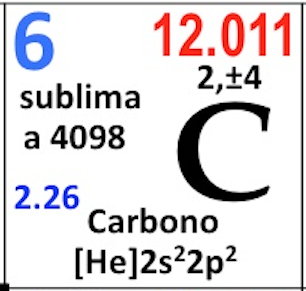
\includegraphics[scale=0.2]{Imagene/carbono.png}
\end{center}

\begin{align}
    \mi{m_c&=\text{partículas}*m_{\text{protón}}}\\
    \mi{&=12.011*(1.67*10^{-27}kg)}\\
    \mi{&=2.004*10^{-26}kg}
\end{align}

Calculando la velocidad en el \textit{selector de velocidades:}
\begin{center}
    

\tikzset{every picture/.style={line width=0.75pt}} %set default line width to 0.75pt        

\begin{tikzpicture}[x=0.75pt,y=0.75pt,yscale=-1,xscale=1]
%uncomment if require: \path (0,350); %set diagram left start at 0, and has height of 350

%Straight Lines [id:da017396953185379815] 
\draw [line width=2.25]    (279.6,149.8) -- (279.6,75.8) ;
\draw [shift={(279.6,71.8)}, rotate = 450] [color={rgb, 255:red, 0; green, 0; blue, 0 }  ][line width=2.25]    (17.49,-5.26) .. controls (11.12,-2.23) and (5.29,-0.48) .. (0,0) .. controls (5.29,0.48) and (11.12,2.23) .. (17.49,5.26)   ;
%Straight Lines [id:da9828083115081834] 
\draw [line width=2.25]    (279.6,149.8) -- (280.54,215.8) ;
\draw [shift={(280.6,219.8)}, rotate = 269.18] [color={rgb, 255:red, 0; green, 0; blue, 0 }  ][line width=2.25]    (17.49,-5.26) .. controls (11.12,-2.23) and (5.29,-0.48) .. (0,0) .. controls (5.29,0.48) and (11.12,2.23) .. (17.49,5.26)   ;
%Shape: Circle [id:dp6020405437570824] 
\draw  [color={rgb, 255:red, 0; green, 0; blue, 0 }  ,draw opacity=1 ][fill={rgb, 255:red, 255; green, 0; blue, 0 }  ,fill opacity=1 ] (275.95,146.15) .. controls (275.95,144.13) and (277.58,142.5) .. (279.6,142.5) .. controls (281.62,142.5) and (283.25,144.13) .. (283.25,146.15) .. controls (283.25,148.17) and (281.62,149.8) .. (279.6,149.8) .. controls (277.58,149.8) and (275.95,148.17) .. (275.95,146.15) -- cycle ;

% Text Node
\draw (294,101.1) node [anchor=north west][inner sep=0.75pt]    {$F_{m}$};
% Text Node
\draw (295,162.1) node [anchor=north west][inner sep=0.75pt]    {$F_{E}$};


\end{tikzpicture}
\end{center}
\begin{align}
    \mi{F_E&=F_m}\\
    \mi{qE&=qvB}\\
\intertext{Despejando para $v$:}
    \mi{v&=\frac{E}{B}}
\end{align}

Calculando el radio:

\begin{center}
    

\tikzset{every picture/.style={line width=0.75pt}} %set default line width to 0.75pt        

\begin{tikzpicture}[x=0.75pt,y=0.75pt,yscale=-1,xscale=1]
%uncomment if require: \path (0,350); %set diagram left start at 0, and has height of 350

%Curve Lines [id:da8247638375638005] 
\draw [color={rgb, 255:red, 255; green, 0; blue, 0 }  ,draw opacity=1 ]   (111,92) .. controls (178.8,91.8) and (180.8,178.8) .. (111.8,178.8) ;
%Straight Lines [id:da6312602290301964] 
\draw    (161.8,138.8) -- (122.8,139.75) ;
\draw [shift={(120.8,139.8)}, rotate = 358.6] [color={rgb, 255:red, 0; green, 0; blue, 0 }  ][line width=0.75]    (10.93,-3.29) .. controls (6.95,-1.4) and (3.31,-0.3) .. (0,0) .. controls (3.31,0.3) and (6.95,1.4) .. (10.93,3.29)   ;

% Text Node
\draw (121,116.1) node [anchor=north west][inner sep=0.75pt]  [font=\small]  {${F_{M}}_{2}$};

\end{tikzpicture}
\end{center}

\begin{align}
    \mi{{F_{M}}_2=qvB&=m\frac{v^2}{R}}\\
    \mi{\implies q\frac{E}{B}B&=m\frac{(\frac{E}{B})^2}{R}}\\
    \intertext{Despejando para $R$:}
    \mi{\implies R&=\frac{m(\frac{E}{B})^2}{qE}}\\
    \mi{&=\frac{m}{q}*\frac{E}{(B)^2}}\\
    \mi{&=\frac{(2.004*10^{-26}kg)(2500 V/m)}{(1,602*10^{-19}C)(0.035T)^2}}\\
    \mi{&\approx 0.255m}
\end{align}



%3----
\textbf{Problema 3}

Una varilla con 0.720 kg de masa y un radio de $6.00 \mathrm{cm}$ descansa sobre dos rieles paralelos (figura) que están separados por un valor $d=12.0 \mathrm{cm}$ y tiene una longitud $L=45.0 \mathrm{cm}$ de largo. La varilla conduce una corriente $I=48.0 \mathrm{A}$ en la dirección que se muestra y rueda por los rieles sin resbalar. Perpendicularmente a la varilla y a los rieles existe un campo magnético uniforme de magnitud 0.240 T. Si parte del reposo, ¿cuál será la rapidez de la varilla cuando se salga de los rieles?\\
\begin{center}
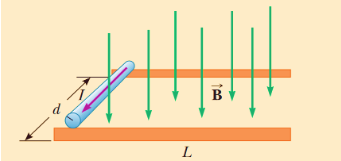
\includegraphics[scale=0.7]{Imagene/1.png}
\end{center}

\textit{Solución}

\begin{center}
    

\tikzset{every picture/.style={line width=0.75pt}} %set default line width to 0.75pt        

\begin{tikzpicture}[x=0.75pt,y=0.75pt,yscale=-1,xscale=1]
%uncomment if require: \path (0,350); %set diagram left start at 0, and has height of 350

%Shape: Circle [id:dp45332953331231374] 
\draw  [line width=2.25]  (270,146.2) .. controls (270,118.92) and (292.12,96.8) .. (319.4,96.8) .. controls (346.68,96.8) and (368.8,118.92) .. (368.8,146.2) .. controls (368.8,173.48) and (346.68,195.6) .. (319.4,195.6) .. controls (292.12,195.6) and (270,173.48) .. (270,146.2) -- cycle ;
%Straight Lines [id:da3024075488146355] 
\draw    (319.4,146.2) -- (417.8,146.79) ;
\draw [shift={(419.8,146.8)}, rotate = 180.34] [color={rgb, 255:red, 0; green, 0; blue, 0 }  ][line width=0.75]    (10.93,-3.29) .. controls (6.95,-1.4) and (3.31,-0.3) .. (0,0) .. controls (3.31,0.3) and (6.95,1.4) .. (10.93,3.29)   ;
%Straight Lines [id:da16547460875054743] 
\draw    (192,200) -- (429.8,195.8) ;
%Straight Lines [id:da8613686837296433] 
\draw  [dash pattern={on 4.5pt off 4.5pt}]  (319.4,146.2) -- (319.4,195.6) ;
%Shape: Circle [id:dp22255941544860325] 
\draw  [fill={rgb, 255:red, 255; green, 0; blue, 0 }  ,fill opacity=1 ] (310.9,197.9) .. controls (310.9,192.87) and (314.97,188.8) .. (320,188.8) .. controls (325.03,188.8) and (329.1,192.87) .. (329.1,197.9) .. controls (329.1,202.93) and (325.03,207) .. (320,207) .. controls (314.97,207) and (310.9,202.93) .. (310.9,197.9) -- cycle ;
%Straight Lines [id:da19904477816453925] 
\draw    (264.8,233.8) -- (305.31,208.07) ;
\draw [shift={(307,207)}, rotate = 507.58] [color={rgb, 255:red, 0; green, 0; blue, 0 }  ][line width=0.75]    (10.93,-3.29) .. controls (6.95,-1.4) and (3.31,-0.3) .. (0,0) .. controls (3.31,0.3) and (6.95,1.4) .. (10.93,3.29)   ;

% Text Node
\draw (301,161.1) node [anchor=north west][inner sep=0.75pt]    {$R$};
% Text Node
\draw (395,120.1) node [anchor=north west][inner sep=0.75pt]    {$F$};
% Text Node
\draw (222,221.1) node [anchor=north west][inner sep=0.75pt]    {$ \begin{array}{l}
pivote\\
\end{array}$};


\end{tikzpicture}
\end{center}
Teniendo en cuenta en lo siguiente:
\begin{itemize}
    \item i – corriente
    \item I - momento de inercia
\end{itemize}
\begin{align}
\intertext{Despejando para la fuerza:}
    \mi{RF&=I\al =I*\frac{a_{cm}}{R}}\\
    \mi{&= (\frac{1}{2}MR^2+MR^2)*\frac{a_{cm}}{R}}\\
    \mi{F&= \frac{3}{2}Ma_{cm}}\\
\intertext{La corriente que circula por la varilla es perpendicular al campo, por lo que se puede asumir:}
    \mi{F&=idB\sin \p }\\
    \mi{&= idB*1}
\intertext{Igualando las ecuaciones:}
    \mi{idB&=\frac{3}{2}Ma_{cm}}\\
    \mi{\implies a_{CM}&=\frac{2idB}{3M}}\\
    \mi{&= \frac{2(48A)(0.12m)(0.24T)}{3(0.72kg)}}\\
    \mi{&= 1.28 m/s^2}
\intertext{Usando cinemática:}
    \mi{V_f^2&=V_0^2+2a\Delta x}\\
    \mi{V_f&=\sqrt{2a\Delta x}}\\
    \mi{&=\sqrt{2(1.28m/s^2)(0.45m)}}\\
    \mi{&\approx 1.07 m/s}
\end{align}

%4---
\textbf{Problema 4}

Veinte bucles de alambre están enrollados estrechamente alrededor de un lápiz redondo de $6.00 \mathrm{mm}$ de diámetro. Luego, el lápiz se coloca en un campo magnético uniforme de $5.00 \mathrm{T}$, como presenta la figura. Si una corriente de $3.00 \mathrm{A}$ está presente en la bobina de alambre, ¿cuál es la magnitud del momento de torsión del lápiz?
\begin{center} 
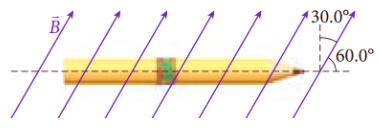
\includegraphics[scale=0.7]{Imagene/2.png}
\end{center}
\textit{Solución}
\begin{align}
    \intertext{El problema requiere que encontremos el torque:}
    \mi{\tau &= iNAB\sin\p}\\
    \mi{&= (3A)(20)\pi (\frac{6*10^{-3} m}{2})^2(5T)\sin(60^{\circ})}\\
    \mi{&=7.346*10^{-3}Nm}
\end{align}

\end{document}